\documentclass[11pt]{exam}

\usepackage[utf8]{inputenc}
\usepackage{hyperref}
\usepackage[spanish]{babel}
\usepackage{graphicx}

\title{Práctica 1}
\author{Laura Rodríguez Navas \\ rodrigueznavas@posgrado.uimp.es}
\date{{\selectlanguage{spanish}\today} }

\pagestyle{plain}

\begin{document}
	
\maketitle

\section*{Ejercicio 1}

\begin{enumerate}
	\item Descargar el código fuente para esta práctica, \textit{softpractica1.zip}, de la página web de la asignatura
	\item Descomprimir el fichero anterior.
	\item Abrir un terminal o consola de comandos y entrar dentro de la carpeta \textit{softpractica1}.
	\item Para empezar vamos a ejecutar GridWorld en el modo de control manual, que utiliza las teclas de flecha (ver Figura \ref{image_1}). \\ \textit{python gridworld.py -m -n 0}	
	\item El objetivo es lograr llegar lo antes posible a la celda etiquetada con un 1, evitando caer en la celda con un -1.
\end{enumerate}

\begin{figure}[h]
	\centering
	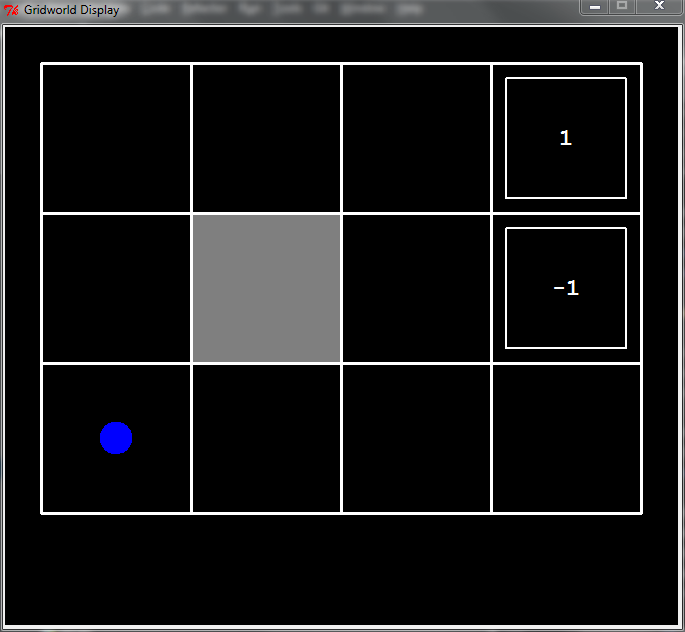
\includegraphics[scale=0.5]{image_1}
	\caption{Interfaz del dominio GridWorld.}
	\label{image_1}
\end{figure}


\subsection*{Preguntas}

\begin{questions}
	
% Pregunta 1
{ \question ¿Cuántas celdas/estados aparecen en el tablero? ¿Cuántas acciones puede ejecutar el agente? Si quisieras resolver el juego mediante aprendizaje por refuerzo, ¿cómo lo harías? 
}

En el tablero aparecen 11 celdas/estado.

El agente puede ejecutar 6 acciones: \textit{north}, \textit{west}, \textit{south}, \textit{east}, \textit{exit} y \textit{done}.

Para resolver el juego mediante el algoritmo Q-Learning: \textbf{TODO}

% Pregunta 2
{ \question Abrir el fichero \textit{qlearningAgents.py} y buscar la clase \textit{QLearningAgent}. Describir los métodos que aparecen en ella.
}

Los métodos que aparecen en la clase \textit{QLearningAgent} son:

\begin{itemize}
	\item \_\_init\_\_: Inicializa la \textit{Q-Table} a partir del fichero \textit{qtable.txt}, es decir, la \textit{Q-Table} se inicializa a cero.
	
	\item readQtable: Lee la \textit{Q-Table} del fichero \textit{qtable.txt}.
	
	\item writeQtable: Escribe la \textit{Q-Table} en el fichero \textit{qtable.txt}.
	
	\item \_\_del\_\_: Llama al método \textit{writeQtable} que escribe el resultado final de la \textit{Q-Table} en el fichero \textit{qtable.txt}.
	
	\item computePosition: Calcula la fila de la \textit{Q-Table} para un estado dado.
	
	\item getQValue: Devuelve el valor $Q(s,a)$ para un estado y una acción dados. De lo contrario, devuelve 0.0, si nunca hemos visto el estado o el valor del nodo $Q$.
	
	\item computeValueFromQValues: Devuelve el valor máximo de $Q(s,a)$ para un estado dado. Este valor se encuentra por encima de las acciones válidas. Si no hay acciones válidas, como en el caso del estado \textit{exit}, devuelve 0.0.
	
	\item computeActionFromQValues: Calcula la mejor acción a realizar para un estado dado. Si no hay acciones válidas, como en el caso del estado \textit{exit}, devuelve \textit{None}.
	
	\item getAction: Calcula la acción a realizar para un estado dado. En caso contrario, con probabilidad \textit{self.epsilon}, elige una acción aleatoria y la mejor acción política. Si no hay acciones válidas, como en el caso del estado \textit{exit}, elige \textit{None} como acción.
	
	\item update: Actualiza la \textit{Q-Table}. El método para un acción dada, observa una recompensa, introduce un estado nuevo (que depende del estado anterior y de la acción dada), y actualiza el valor $Q(s,a)$. 
	
	Si el nuevo estado introducido es el estado \textit{exit}, se sigue la regla:
	
	\begin{center}
		$Q(state,action) <- (1-self.alpha) * Q(state,action) + self.alpha * (reward + 0)$
	\end{center}

	De lo contrario, si el nuevo estado introducido no es el estado \textit{exit}, se sigue la regla:
	
	\begin{center}
		$Q(state,action) <- (1-self.alpha) * Q(state,action) + self.alpha * (reward + self.discount * max a' Q(nextState, a'))$
	\end{center}
	
	\item getPolicy: Devuelve la mejor acción de la \textit{Q-Table} para un estado dado.
	
	\item getValue: Devuelve el valor $Q(s,a)$ más alto para un estado dado.
		
\end{itemize}

% Pregunta 3
{ \question Ejecuta ahora el agente anterior con: \\ \textit{python gridworld.py -a q -k 100 -n 0}}

A diferencia de la primera ejecución, en esta le indicamos el tipo de agente (q) y el número de episodios del MDP a ejecutar (100).

\begin{figure}[h]
	\centering
	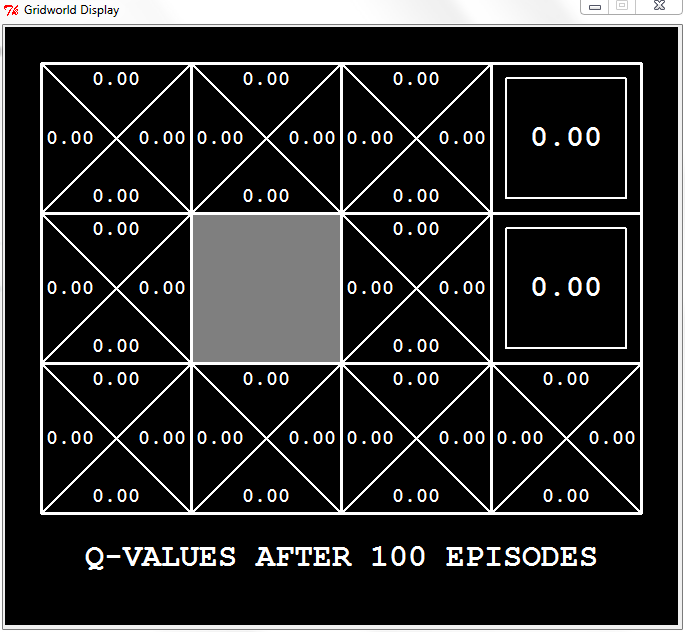
\includegraphics[scale=0.5]{image_2}
	\caption{Interfaz del dominio GridWorld.}
	\label{image_2}
\end{figure}

% Pregunta 4
{ \question ¿Qué información se muestra en el laberinto? ¿Qué aparece por terminal cuando se realizan los movimientos en el laberinto? 
}

Si observamos la Figura \ref{image_2} vemos que la información que se muestra son los valores de $Q(s,a)$. 

En la terminal, cuando se realizan los movimientos en el laberinto, vemos que aparecen los siguientes valores:

\begin{itemize}
	\item La posición (x, y) donde empieza el estado. Por ejemplo: (2, 1).
	\item La acción tomada. Por ejemplo: \textit{east}.
	\item La posición (x, y) donde acaba el estado. Por ejemplo: (3, 1).
	\item La recompensa obtenida. Por ejemplo: 0.0, en este caso no ha habido recompensa.
\end{itemize}

% Pregunta 5
{ \question ¿Qué clase de movimiento realiza el agente anterior?}

% El agente siempre que decida moverse en una dirección, lo hace en esa dirección con probabilidad 1 (se mueve una posición).

% Pregunta 6
{ \question ¿Se pueden sacar varias políticas óptimas? Describe todas las políticas óptimas para este problema.}

% Pregunta 7
{ \question Escribir el método \textit{update} de la clase \textit{QLearningAgent} utilizando las funciones de actualización del algoritmo \textit{Q-Learning}. Para ello, inserta el código necesario allí donde aparezca la etiqueta INSERTA TU CÓDIGO AQUÍ siguiendo las instrucciones que se proporcionan, con el fin de conseguir el comportamiento deseado. }

% Pregunta 8
{ \question Establece en el constructor de la clase \textit{QLearningAgent} el valor de la variable \textit{epsilon} a 0,05. Ejecuta nuevamente con: \\ \textit{python gridworld.py -a q -k 100 -n 0} \\ ¿Qué sucede?
}

% Pregunta 9
{ \question Después de la ejecución anterior, abrir el fichero \textit{qtable.txt}. ¿Qué contiene?}

\end{questions}

\section*{Ejercicio 2}

En el ejercicio anterior, siempre que el agente decidía moverse hacia una dirección se movía en esa dirección con probabilidad 1. Es decir, se trataba de un MDP determinista. Ahora vamos a crear un MDP estocástico:

\begin{questions}

% Pregunta 1
{ \question Ejecuta y juega un par de partidas con el agente manual: \\ \textit{python gridworld.py -m -n 0.3} \\ ¿Qué sucede? ¿Crees que el agente \textit{QLearningAgent} será capaz de aprender en este nuevo escenario?
}

% Pregunta 2
{ \question Reiniciar los valores de la tabla Q del fichero \textit{qtable.txt}. Para ello ejecutar desde el terminal: \\ \textit{cp qtable.ini.txt qtable.txt}
}

% Pregunta 3
{ \question Ejecutar el agente \textit{QLearningAgent}: \\ \textit{python gridworld.py -a q -k 100 -n 0.3}}

% Pregunta 4
{ \question Tras unas cuantos episodios, ¿se genera la política óptima? Y si se genera, ¿se tarda más o menos que en el caso determinista?
}

\end{questions}

\end{document}
